% --------------------------------------------------------------
% Abhi's Standard math Preamble.
% --------------------------------------------------------------
 
\documentclass[12pt]{article}
 
%Math Packages
\usepackage[margin=1in]{geometry} 
\usepackage{amsmath,amsthm,amssymb,mathrsfs,bm}
\usepackage{mathtools}
\usepackage{xfrac}
\usepackage{commath}
\usepackage{minted}
\usepackage{enumerate}
\usepackage{fancyhdr}
\usepackage{esint}
\usepackage{algorithm}
\usepackage{algpseudocode}
\usepackage{qtree}
\usepackage{epigraph}
\usepackage{centernot}
\usepackage{float}


 
%Fonts
%\usepackage[sc,osf]{mathpazo}   % With old-style figures and real smallcaps.
%\usepackage{lmodern}
%\usepackage{eulervm}

\DeclareMathOperator{\sign}{sgn}

%Math commands
% Mathematical Fields
\newcommand{\R}{\mathbb{R}}
\newcommand{\N}{\mathbb{N}}
\newcommand{\Q}{\mathbb{Q}}
\newcommand{\Z}{\mathbb{Z}}
\newcommand{\C}{\mathbb{C}}
%Divides and Not Divides
\newcommand{\divides}{\bigm|}
\newcommand{\ndivides}{%
  \mathrel{\mkern.5mu % small adjustment
    % superimpose \nmid to \big|
    \ooalign{\hidewidth$\big|$\hidewidth\cr$\nmid$\cr}%
  }%
}
%Limit as n -> inf
\newcommand{\limty}{\lim_{n \to \infty}}
%sum from n=1 \to inf
\newcommand{\sumty}{\sum_{n = 1}^\infty}

\newcommand{\lindelof}{Lindel\={o}f }

\theoremstyle{definition}
\newtheorem*{lemma*}{Lemma}
\newtheorem*{definition*}{Definition}
 
\begin{document}
 
% --------------------------------------------------------------
%                         Start here
% --------------------------------------------------------------

 
\title{Algorithms Topics Review}%replace X with the appropriate number
\author{Abhijit Chowdhary\\ %replace with your name
Fundamental Algorithms \\
Prof. Siegel} %if necessary, replace with your course title

\maketitle

\epigraph{Beware of bugs in the below code: I have only proved it correct, not
tried it.}{\textit{Donald Knuth}}

\tableofcontents
\pagebreak

\section{Asymptotics and Recurrences}

% MATH REVIEW SUBSECTION |-----------------------------------------------------|

\subsection{Math Review}

Before we talk about asymptotics and recurrences, we quickly review the
logarithmic function $\log$.

\begin{definition*}
We define the \textbf{logarithm} to be the opposite of exponentiation, i.e. we
say that $\log_b(x) = y$ exactly if $b^y = x$. For example $\log_2(64) = 6$,
since $64 = 2^6$. 
\end{definition*}

Here's a couple useful properties of the $\log$ that you will use in this
section extensively.

\begin{enumerate}[(1)]

\item Product $\to$ Summation: $\log_b(xy) = \log_b(x) + \log_b(y)$.

\begin{proof}

By definition, we know that $b^{\log_b(xy)} = xy$. However, also notice that $x
= b^{\log_b(x)}$ and $y = b^{\log_b(y)} \implies xy = b^{\log_b(x)}b^{\log_b(y)}
= b^{\log_b(x) + \log_b(y)} \implies b^{\log_b(xy)} = b^{\log_b(x) + \log_b(y)}$.

\end{proof}

\item Quotient $\to$ Subtraction: $\log_b \left( \frac{x}{y} \right) = \log_b(x)
- \log_b(y)$. 

\begin{proof}
This can be seen using the previous identity, and just taking $y \mapsto
\frac{1}{y}$, and noticing that $\frac{1}{y} = \frac{1}{b^{\log_b(y)}} =
b^{-\log_b(y)}$.
\end{proof}

\item Power $\to$ Scalar Multiplication: $\log_b(x^p) = p\log_b(x)$.

\begin{proof}

By defintion:

$$
x = b^{\log_b(x)} \implies x^p = \left(b^{\log_b(x)}\right)^p = b^{p\log_b(x)} 
$$

Therefore it must be true that $\log_b(x^p) = p\log_b(x)$.

\end{proof}

\item Change of Base: $\log_b(x) = \frac{\log_k(x)}{\log_k(b)}$.

\begin{proof}

Starting from $x = b^{\log_b(x)}$, we can take $\log_k$ of both sides to
recieve:

$$
\log_k(x) = \log_k b^{\log_b(x)} = \log_b(x) \log_k(b)
$$

Therefore, dividing through by $\log_k(b)$ gives us the desired identity.

\end{proof}

\end{enumerate}

% ASYMPTOTICS SUBSECTION |-----------------------------------------------------|

\subsection{Asymptotics Analysis}

In the analysis of algorithms, one of our goals is to classify growth of the

runtime and storage complexity of functions. To do so, it's in our interest to
examine the limiting behavior of functions, i.e. when our input becomes large
what does our function do. To this end we introduce Big O notation.

\subsubsection{Big O notation}

Big O notation exists to describe the limiting behavior of a function, and us
Computer Scientists use it to classify algorithms in terms of their input size
$n$. Due to this, from this point onwards all functions we define are
non-negative. 

We give both the informal and formal definition of a couple different
useful characterizations. Let $f,g : \R \to \R$ be two functions.

\begin{itemize}

\item Upper bound: $\mathcal{O}$.

\begin{definition*}
Informally, we say that $f(x) = \mathcal{O}(g(x))$ if $ f(x) \leq cg(x)$, $c$
some constant, for sufficiently large $x$. 

Formally, $f(x) = \mathcal{O}(g(x))$ iff:

$$
\limsup_{x \to \infty} \abs{\frac{f(x)}{g(x)}} < \infty
$$

For example, $n^2 = \mathcal{O}(n^2)$ and $n^2 = \mathcal{O}(n^5)$ but $n^2 \neq
\mathcal{O}(n)$. To highlight the sufficiently large $x$ portion, notice that it
is true that $n^2 = \mathcal{O}(n^3 - n^2)$ ($n^3 - n^2 > n^2, \forall n > 2$.)

\end{definition*}

\item Lower Bound: $\Omega$.

\begin{definition*}

Informally, we say that $f(x) = \Omega(g(x))$ if and only if $g(x) =
\mathcal{O}(f(x))$, or that $f(x) \geq cg(x)$.

Formally $f(x) = \Omega(g(x)) \iff \liminf_{n \to \infty}
\abs{\frac{f(n)}{g(n)}} > 0$.

\end{definition*}

\item Tight bound: $\theta$.

\begin{definition*}

We say that $f(x) = \theta(g(x))$ if $f(x) = \mathcal{O}(g(x))$ and $f(x) =
\Omega(g(x))$. Another way to say this is that $\exists c \in \R$ such that
$\frac{1}{c} g(x) \leq f(x) \leq cg(x)$, for sufficiently large enough $x$.

Formally we must have that:

$$
\limsup_{x \to \infty} \abs{\frac{f(x)}{g(x)}} \in \R_{> 0}
$$

To those that care, notice that having $f(x) = \mathcal{O}(g(x))$ and
$\Omega(g(x)) \centernot \implies \lim_{x \to \infty} \abs{\frac{f(x)}{g(x)}}$ exists.
Instead $\liminf$ and $\limsup$ may converge to different values.

So for example, $n^2 = \theta(n^2)$ but $n^2 \neq \theta(n)$ and $\neq
\theta(n^3)$.

\end{definition*}

\end{itemize}

\subsubsection{Properties of Big O}

There's a couple of useful properties of Big O that are good to know. Let $f_1 =
\theta(g_1)$ and $f_2 = \theta(g_2)$.

\begin{enumerate}[(1)]

\item Product: $f_1f_2 = \theta(g_1g_2)$. In addition $f \theta(g) =
\theta(fg)$.

\item Sum: $f_1 + f_2 = \theta(g_1 + g_2)$. In particular if $f_1 =
\mathcal{O}(g)$ and $f_2 = \mathcal{O}(g)$ then $f_1+f_2 = \mathcal{O}(g)$.

\item Scalar multiplication: $\theta(kg) = \theta(g)$ supposing $k \neq 0$. In
addition $kf_1 = \theta(g_1)$.

\item Elephant concept: Suppose $\max(g_1, g_2) = g_1$. Then $\theta(g_1 + g_2)
= \theta(g_1)$. NOTE that this does not imply that $\theta(g_1g_2) =
\theta(g_1)$. Counterexample is $g_1(n) = g_2(n) = n$. You can think about this
like $\theta$ takes summation to maximization.

\end{enumerate}

\subsubsection{Time Complexity Comparison}

Typically for problems where we want to compare which function grows faster
asymptotically, we really want to see at large $x$, which one dominates. Our
main strategy to do this, is to reduce these functions down to functions which
are more easily compared, which I call the time complexity classes. See the time
complexity chart in the figures section for a good table of a commmon few which
you should remember. 

Take for examples:

\begin{enumerate}[(1)]

\item $2^n$ versus $n^2$.

\begin{proof}[Solution]

It's clear that $2^n$ is exponential, which grows faster than $n^2$ which is
polynomial.

\end{proof}

\item $n^{\log(n)}$ versus $n^{100}$.

\begin{proof}[Solution]

The left hand function is somewhere above polynomial due to the power being an
increasing function of $n$. Therefore, it grows faster than $n^{100}$.

\end{proof}

\item $n^{1/\log_2(n)}$ versus $2$.

These are strange to compare, since we aren't sure what class the left hand
function falls in. To try to fit it to something we understand, we remember that
the logarithm takes powers to scalar multiplcation, so then we notice:

$$
\log_2(n^{1/\log_2(n)}) = \frac{1}{\log_2(n)} \log_2(n) = 1
$$

But also $\log_2(2) = 1$. Therefore we find that these functions are actually
equal in terms of asymptotic growth.

\end{enumerate}

% RANDOMIZED FUNCTION SUBSECTION |---------------------------------------------|

\subsection{Algorithm $\to$ Recurrence}

Here we want to examine how to turn recursive code into reucurrences
characterizing their properties. We do this by example.

\subsubsection{Fibbonacci Sequence}

\begin{algorithmic}[1]
\Procedure{F}{$n$}\Comment{$a_1 = 1, a_2 = 1, a_n = a_{n-1}+a_{n-2}$}
	\If{$n \leq 2$}
		\State Return $1$
	\Else
		\State Return $F(n-1)+F(n-2)$
	\EndIf
\EndProcedure
\end{algorithmic}

Suppose we want to characterize the runtime of the above algorithm using a
recurrence equation. The idea is that we count the work per level, and add it.
Letting $G(n)$ characterize the runtime of $F(n)$.

\begin{algorithmic}[1]
\Procedure{F}{$n$}
	\If{$n \leq 2$} \Comment{$\theta(1)$}
		\State Return $1$ \Comment{$\theta(1)$}
	\Else \Comment{$\theta(1)$}
		\State Return $F(n-1)+F(n-2)$ \Comment{$G(n-1)+G(n-2) + \theta(1)$}
	\EndIf \Comment{$\theta(1)$}
\EndProcedure
\end{algorithmic}

Notice that $\theta(1)$ summed a constant number of times is still $\theta(1)$,
therefore we have:

$$
G(n) = \begin{cases}
\theta(1) & n \leq 2 \\
\theta(1) + G(n-1) + G(n-2) & \text{otherwise}
\end{cases}
$$

For characterizing things that aren't work, i.e. how many times the $-1$
operation happens in the above code, we can do a similar process. Let $H(n)$
characterize the number of $-1$ operations in $F(n)$. Then:

\begin{algorithmic}[1]
\Procedure{F}{$n$}
	\If{$n \leq 2$} \Comment{$0$}
		\State Return $1$ \Comment{$0$}
	\Else \Comment{$0$}
		\State Return $F(n-1)+F(n-2)$ \Comment{$H(n-1)+H(n-2) + 1$}
	\EndIf \Comment{$0$}
\EndProcedure
\end{algorithmic}

Therefore:

$$
H(n) = \begin{cases}
0 & n \leq 2 \\
1 + H(n-1) + H(n-2) & \text{otherwise}
\end{cases}
$$

\subsubsection{Merge Sort}

Let $F(n)$ characterize the work of Merge Sort on an array of length $n$. Then:

\begin{algorithmic}[1]
\Procedure{Mergesort}{$A$ : Array}
	\State Let $n = len(A)$.
	\If{$n = 1$} \Comment{$\theta(1)$}
		\State Return $A$ \Comment{$\theta(1)$}
	\EndIf \Comment{$\theta(1)$}
	\State $B \gets A[1... \lfloor n/2 \rfloor]$ \Comment{$\theta(1)$}
	\State $C \gets A[\lceil n/2 \rceil ... n]$ \Comment{$\theta(1)$}
	\State $Mergesort(B), Mergesort(C)$ \Comment{$F(\lfloor n/2 \rfloor) +
	F(\lceil n/2 \rceil)$}
	\State Return $Merge(B,C)$ \Comment{$\theta(n)$} 
\EndProcedure
\end{algorithmic}

Therefore we have:

$$
F(n) = \begin{cases}
\theta(1) & n = 1 \\
\theta(n) + F(\lfloor n/2 \rfloor) + F(\lceil n/2 \rceil) & \text{otherwise}
\end{cases}
$$

Similarily we can do this for $H(n)$ characterizing storage constraints, but
I'll leave that as exercise.

\subsubsection{Randomized Algorithms}

A classic Siegel question is to characterize various facets of the randomized
algorithm:

\begin{algorithmic}[1]
\Procedure{Rand}{$n$}
	\If{$n \leq 1$} 
		\State Return 0 
	\EndIf 
	\State Let $x \gets 1, 2$ or $3$ with probabilities $1/2, 1/3, 1/6$
	respectively.
	\If{$x = 1$}
		\State Return $2Rand(n)$
	\ElsIf{$x = 2$}
		\State Return $7Rand(n-1) + 12Rand(n-2)$
	\Else
		\State Return $nRand(n-1)$
	\EndIf
\EndProcedure
\end{algorithmic}

Define function $F, G, H$ which characterize runtime, exact value returned, and
number of times $x \gets 3$ respectively. The trick to characterizing the above,
is simply to take whatever happens inside of an if statement and multiply it by
the probability of the event occuring. So:

\begin{align*}
F(n) & = \begin{cases}
\theta(1) & n \leq 1 \\
\theta(1) + \frac{1}{2} (\theta(1) + F(n)) + \frac{1}{3} (\theta(1) + F(n-1) +
F(n-2)) + \frac{1}{6}( \theta(1) + F(n-1) ) & \text{otherwise}
\end{cases} \\
G(n) & = \begin{cases}
0 & n \leq 1 \\
\frac{1}{2} (2H(n)) + \frac{1}{3} (7H(n-1) + 12H(n-2)) + \frac{1}{6}( nH(n-1) )
& \text{otherwise}
\end{cases} \\
H(n) & = \begin{cases}
0 & n \leq 1 \\
\frac{1}{2} (0 + H(n)) + \frac{1}{3} (0 + H(n-1) + H(n-2)) + \frac{1}{6}(1 +
H(n-1) ) & \text{otherwise}
\end{cases} \\
\end{align*}

This always appears on the exam.

% Solving RECURRENCES SUBSECTION |---------------------------------------------|

\subsection{Solving Recurrences}

Ok, so now that we know how to characterize certain aspects of recursive code
using recurrences, one might ask, how do we solve recurrences? The idea stems
behind something called the tree method. For example, consider the recurrence
equation:

$$
f(n) = \begin{cases}
1 & n = 1 \\
n + 2f(n/3) & \text{otherwise}
\end{cases}
$$

Here we call $n$ the work function, $3$ the decay rate, and $2$ the branching
factor.

What we do to solve this is \textit{unroll} the recursive term over and over
again. We represent each unrolling as a new level of the tree, so it may look
like:

\Tree
[.$n$
	[.$n/3$ 
		[.$n/9$ $\vdots$ $\vdots$ ] 
		[.$n/9$ $\vdots$ $\vdots$ ] 
	]
	[.$n/3$ 
		[.$n/9$ $\vdots$ $\vdots$ ] 
		[.$n/9$ $\vdots$ $\vdots$ ] 
	]
]

The top level looks like $n + 2f(n/3)$, but then we unroll $f(n/3)$ to $n/3 +
2(n/9)$, which is our second level. To then figure out what our summation totals
to, we sum accross the level, and then downward. In the above example, the first
level totals to $n$, the second to $(2/3)n$, the third to $(4/9)n$, etc. In
fact, we will find that in general the $j$th level will sum to
$\frac{2^j}{3^j}n$; this is guarenteed by the unrolling. But what about the leaf
level?

In general, we have to examine the leaf level seperately, because the recurrence
defines something different for it. Here, our recurrence says that each leaf has
cost $1$. Looking at our tree, we see that at each level the number of vertices
doubles (powers of branching factor), therefore at the leaf level $k$ we must
have $2^k$ leaves. Each costs 1, therefore the contribution from the leaf level
is $2^k$.

Therefore our final
total actually looks something like $n + \frac{2}{3} n + \frac{2^2}{3^n} n +
\dots + \frac{2^{k-1}}{3^{k-1}}n + 2^k$, for some stopping point $k$. Let's find
$k$.

$k$ is determined by the point we can \textit{unroll} no longer, i.e. the decay
rate has been applied sufficiently enough times such that we get down to our
base case, $1$. In other words, we want to solve for $k$ where:

$$
\frac{n}{3^k} = 1 \implies n = 3^k \implies k = \log_3(n)
$$

Since we choose $n$ a power of $3$, we find that $k$ is an integer like we
wanted it to be. Then, we can write our final answer as:

$$
f(n) = n \left(1 + \frac{2}{3} + \frac{2^2}{3} + \dots +
\left(\frac{2}{3}\right)^{\log_3(n)-1} \right) + 2^{\log_3(n)}
$$

We make one note here about the leaf level. Notice that we can say:

$$
2^{\log_3(n)} = \frac{n}{n} 2^{\log_3(n)} = n
\frac{2^{\log_3(n)}}{3^{\log_3(n)}} = n \left( \frac{2}{3} \right)^{\log_3(n)}
$$

This looks exactly like our pattern! What's happening? What we've discovered is
that our leaf level \textit{obeys} our recurrence, and I claim that this is in
general true if the work at the level matches the work function. For example,
the work function $w(n)$ is $n$ here. The base case is at $n = 1$, therefore
looking at $w(1)$ we see it's $1$. \textit{This matches our base case}, i.e.
that at $n = 1, f(n) = 1$. Whenever this happens, it's unecessary to compute the
leaf level seperately, and we can pull it into our summation. Rough reasoning
is that it's modeled perfectly by the recurrence. If we had it that when $n =
1, f(n) = 5$, we could not do this. Therefore we can write:

$$
f(n) = n \left(1 + \frac{2}{3} + \frac{2^2}{3} + \dots +
\left(\frac{2}{3}\right)^{\log_3(n)} \right) 
$$

Let's solve a couple different types of common recurrences you might see.

\subsubsection{Basic Recurrences}

\begin{enumerate}[(1)]

\item Solve the recurrence:

$$
A(n) = \begin{cases}
1 & n = 1 \\
n + 2A(n/2) & \text{otherwise}
\end{cases}
$$

\begin{proof}[Solution]

For this we have work function $f(n) = n$, decay rate $2$ and branching factor
$2$. The tree we draw looks like:

\Tree
[.$n$
	[.$n/2$ 
		[.$n/4$ $\vdots$ $\vdots$ ] 
		[.$n/4$ $\vdots$ $\vdots$ ] 
	]
	[.$n/2$ 
		[.$n/4$ $\vdots$ $\vdots$ ] 
		[.$n/4$ $\vdots$ $\vdots$ ] 
	]
]

Summing across, we come across the surprising fact that each level sums to $n$.
This is roughly because the decay rate and the branching factor cancel each
other out. In general, we find this to be true when $f(\delta(n)) = \beta$ where
$\beta$ is the branching factor and $\delta$ is the decay rate as a function of
$n$ (can you see why?). Ok, so now considering the tree, we can ask how many
terms are there? Recall this is solving for $\frac{n}{2^k} = 1 \implies k =
\log_2(n)$. This tells us that there must be $\log_2(n) + 1$ levels ($k$ tells
us $k$th level, but count starting from $0$). Finally we notice that $f(1) =
A(1)$, which implies that we don't have to do the leaf level seperately.
Therefore our solution is: 

$$
A(n) = n + n + \dots + n = n( \text{Number of levels}) = n(log_2(n)+1)
$$

\end{proof}

\item Solve the reucrrence:

$$
B(n) = \begin{cases}
5, & n = 1 \\
n + 2B(n/2), & \text{otherwise}
\end{cases}
$$

\begin{proof}[Solution]
The difference between this one at the last one is the leaf level. Here we have
that $B(1) \neq f(1)$, which implies we need to compute the leaf level
seperately. There are $2^{\log_2(n)} = n$ leaves, and each has work $5$, which
implies that the leaf level cost is $5n$. Therefore we can write our answer as:
$$
B(n) = nlog_2(n) + 5n
$$
\end{proof}

\subsubsection{Changing the Leaf Level}

What if we have a recurrence like:

$$
C(n) = \begin{cases}
8, & n = 8 \\
n + 3C(n/2), \text{otherwise} 
\end{cases}
$$

In this case what's strange is that we've changed when we enter the leaf level.
The tree method, however, handles this perfectly. Before we asked when
$\frac{n}{b^k} = 1$ where $b$ was the decay rate. Here the base case is when $n
= 8$, so we instead ask $\frac{n}{2^k} = 8 = 2^3 \implies k = \log_2(n) - 3$.
Then the problem is solved in the same exact manner as in the basic recurrences.

\subsubsection{Multiple Decay Rates}

What happens if we have a recurrence like:

$$
D(n) = \begin{cases}
1, & n = 1 \\
n + D(n/2) + D(n/3), & \text{otherwise}
\end{cases}
$$

What we lose is the guarentee that all leaves live on the same level. In fact,
the end of the \textit{unrolling} will come sooner for the harsher decay rate,
and later for the kinder decay rate. In $D(n)$, we see that $\frac{n}{2^k} \to_k
1$ slower than $\frac{n}{2^k} \to_k 1$. To resolve this problem, what we do is
approximate; we say that our leaf level $k$ lives somewhere between the leaf
level defined by $2$ and $3$.

If we follow the decay rate $2$ all of the way down, we know that our leaf level
is $k_2 = \log_2(n)$. If we follow $3$, similarily we will recieve $k_3 =
\log_3(n)$. We say that our "leaf level" lives between these two, or $\log_3(n)
\leq k \leq \log_2(n)$.

Then to solve our problem we have the tree:

\Tree
[.$n$
	[.$n/2$ 
		[.$n/4$ $\vdots$ $\vdots$ ] 
		[.$n/6$ $\vdots$ $\vdots$ ] 
	]
	[.$n/3$ 
		[.$n/6$ $\vdots$ $\vdots$ ] 
		[.$n/9$ $\vdots$ $\vdots$ ] 
	]
]

We find that our summation looks like:

$$
D(n) \approx n\left[ 1 + \frac{5}{6} + \frac{5^2}{6^2} + \dots +
\left(\frac{5}{6}\right)^k \right],\quad  \log_3(n) \leq k \leq \log_2(n)
$$

\subsubsection{Strange Decay Rates}

What happens if we have a recurrence like:

$$
E(n) = \begin{cases}
1, & n = 1 \\
1 + 2E(\delta(n)), & \text{otherwise}
\end{cases}
$$

Lots of people get stuck on this, but I claim that our tree method handles this
perfectly. The tree itself looks like:

\Tree
[.$1$
	[.$1$ 
		[.$1$ $\vdots$ $\vdots$ ] 
		[.$1$ $\vdots$ $\vdots$ ] 
	]
	[.$1$ 
		[.$1$ $\vdots$ $\vdots$ ] 
		[.$1$ $\vdots$ $\vdots$ ] 
	]
]

The real question is, where is the leaf level? Before we asked for decay rate
$\delta(n) = \frac{n}{b}$, how many times do we have to apply it to get down to
the base case. This formulated as $\frac{n}{b^k} = 1 \implies k = \log_b(n)$.
Our question in general is for what $k$ does $\delta^k(n) = 1$, where $k$ isn't
a power but repeated function compositions. For example if $\delta(n) = n-1$,
then we would be asking $n - k(-1) = 1 \implies k = n-1$. 

\end{enumerate}

\section{Dynamic Programming}

Dynamic programming is a technique from optimization field, specally it's a
method to solve problem if the problem exhibits \textbf{optimal substructure}
and \textbf{overlapping subproblems}.

\begin{definition*}

A problem is said to have \textbf{optimal substructure} if it can be constructed
from optimal solutions of its subproblems. 

For an example, suppose $T$ a tree and consider the problem where $\forall v \in
T$, you want to compute a field $\min$ such that $\min[v] = \min\{w.val : w \in
ST(v)\}$ where $ST(v)$ denotes the subtree rooted by $v$. This problem exhibits
optimal substructure, as for arbitrary vertex $v$, you have $\min[w]$ computed
for all $w \in Children[v]$, then you can construct $\min[v]$ as the minimum of
your childrens answers and your own.

\end{definition*}

\begin{definition*}

A problem is said to have \textbf{overlapping subproblems} if the problem can be
broken down into subproblems which are reused several times.

For an example, consider the Fibonnacci number sequence $a_n = a_{n-1} +
a_{n-2}, a_2 = a_1 = 1$. Consider the value $a_5$. Notice that we can express it
as a graph (see figure 2) with many incoming edges (in particular a DAG).
Whereas problems with optimal substructure but not overlapping subproblems look
like the problem $\min[v]$ problem, and can be modeled by trees.

\end{definition*}

The idea behind the dynamic programming problems we deal with is that if we
remember problems as we do it, we can elimate the "overlapping" problems and
reduce our computational cost as much as possible.

We've discussed three problems that we call "representative" of a lot of dynamic
programming techniques: GCD, Woodcut, and Matrix Chain. We find that many
dynamic programming problems reduce down to similar techniques needed to solve
these. In this section we discuss how to tackle these problems fully, but before
that we introduce \textbf{memoization}.

\subsection{Memoization through Fibbonacci}

As discussed above, the Fibbonacci sequence $F_n = F_{n-1} + F_{n-2}, F_2 = F_1
= 1$, is a prime example of a dynamic programming problem, since it has both
optimal substructure and overlapping subproblems. Using the recurrence
relationship defined above we can write recursive code to solve this problem:

\begin{algorithmic}[1]
\Procedure{F}{$n$}\Comment{$a_1 = 1, a_2 = 1, a_n = a_{n-1}+a_{n-2}$}
	\If{$n \leq 2$}
		\State Return $1$
	\Else
		\State Return $F(n-1)+F(n-2)$
	\EndIf
\EndProcedure
\end{algorithmic}

However, if we were to run just this we would find ourselves choked by the
runtime cost almost immediately. This is a consequence of the overlapping
subproblems portion of Fibbonacci, i.e. we're repeatedly computing the same
pieces of data. How do we resolve this? We implement \textbf{memoization}.

\begin{definition*}
\textbf{Memoization} is an optimization technique where we store and cache the
results of expensive function calls. The idea is that if we want to compute said
function again, we look in our cache first. (Memoization $\gets$ making a memo.)
\end{definition*}

Let's take a look at this implemented in the Fibbonacci sequence.

\begin{algorithmic}[1]
\State Let Memo[1..n] be a integer valued array initialized to $-1$.
\Procedure{F}{$n$}\Comment{Recursive or top down}
	\If{$n \leq 2$}
		\State Return $1$.
	\ElsIf{$Memo[n] \neq -1$} \Comment{If we have computed $n$, use that result}
		\State Return $Memo[n]$. 
	\Else \Comment{Otherwise, compute it, store it, and return it.}
		\State $Memo[n] = F(n-1)+F(n-2)$.
		\State Return $Memo[n]$. 
	\EndIf
\EndProcedure
\end{algorithmic}

We can also implement this iteratively using a lookup table:

\begin{algorithmic}[1]
\Procedure{F}{$n$}\Comment{Iterative or bottom up}
	\State Let Memo[1..n] be a integer valued array.
	\State Let $Memo[1], Memo[2] = 1$.
	\For{$i = 3 \to n$}
		\State $Memo[i] = Memo[i-1] + Memo[i-2]$
	\EndFor
\EndProcedure
\end{algorithmic}

Without the memoization table, our runtime was exponential, but what about now?
It's clear by the iterative version that our usage of memoization brings us to
$\theta(n)$ work, which is basically a night and day difference. In general we
can examing the new runtime of our dynamic programming problem by looking at the
memoization table, and trying to figure out how long it would take to fill it.

\subsection{Greatest Common Subsequence}

The problem is as follows: Suppose you are given two sequence $A$ and $B$. Your
objective is to find a subsequence $S \subseteq A, B$ such that the length of
$S$ is maximized. This is a classic problem for applications in revision
control, the diff utility on your computer, and many more NLP like reasons.

$$
GCS(i,j) = \begin{cases}
0, & ij = 0 \\
1 + GCS(i-1,j-1), & A[i] = A[j] \\
\max(GCS(i-1,j),GCS(i,j-1)), & \text{otherwise}
\end{cases}
$$

\begin{algorithm}
\begin{algorithmic}[1]
\State Let $A[1..n]$ and $B[1..m]$ be two character arrays.
\Procedure{GCS}{$i,j$}
	\If{$ij = 0$}
		\State Return $0$.
	\ElsIf{$A[i] = B[j]$}
		\State Return $1 + GCS(i-1,j-1)$.
	\Else 
		\State Return $\max(GCS(i-1,j),GCS(i,j-1))$.
	\EndIf
\EndProcedure
\end{algorithmic}
\end{algorithm}
\begin{algorithm}
\begin{algorithmic}[1]
\State Let $A[1..n]$ and $B[1..m]$ be two character arrays.
\State Let $Memo[1..n,1..m]$ be a 2d array initialized to $-1$.
\Procedure{GCS}{$i,j$}
	\If{$ij = 0$}
		\State Return $0$.
	\ElsIf{$Memo[i,j] \neq -1$}
		\State Return $Memo[i,j]$.
	\ElsIf{$A[i] = B[j]$}
		\State $Memo[i,j] = 1 + GCS(i-1,j-1)$.
	\Else 
		\State $Memo[i,j] = \max(GCS(i-1,j),GCS(i,j-1))$.
	\EndIf
	\State Return $Memo[i,j]$.
\EndProcedure
\end{algorithmic}
\end{algorithm}
\begin{algorithm*}
\begin{algorithmic}[1]
\State Let $A[1..n]$ and $B[1..m]$ be two character arrays.
\State Let $Memo[1..n,1..m]$ be a 2d array initialized to $-1$.
\State Let $Decisions[1..n,1..m]$ be a 2d array.
\Procedure{GCS}{$i,j$}
	\If{$ij = 0$}
		\State Return $0$.
	\ElsIf{$Memo[i,j] \neq -1$}
		\State Return $Memo[i,j]$.
	\ElsIf{$A[i] = B[j]$}
		\State $Memo[i,j] = 1 + GCS(i-1,j-1)$.
		\State $Decisions[i,j] = (i-1,j-1)$.
	\Else 
		\State $v_1, v_2 = GCS(i-1,j), GCS(i,j-1)$.
		\If{$v_1 > v_2$}
			\State $Memo[i,j] = v_1$.
			\State $Decisions[i,j] = (i-1,j)$.
		\Else
			\State $Memo[i,j] = v_2$.
			\State $Decisions[i,j] = (i,j-1)$.
		\EndIf
	\EndIf
	\State Return $Memo[i,j]$.
\EndProcedure
\end{algorithmic}
\end{algorithm*}


\section{Figures}

\subsection{Common Time Complexities}
\begin{figure}[H]
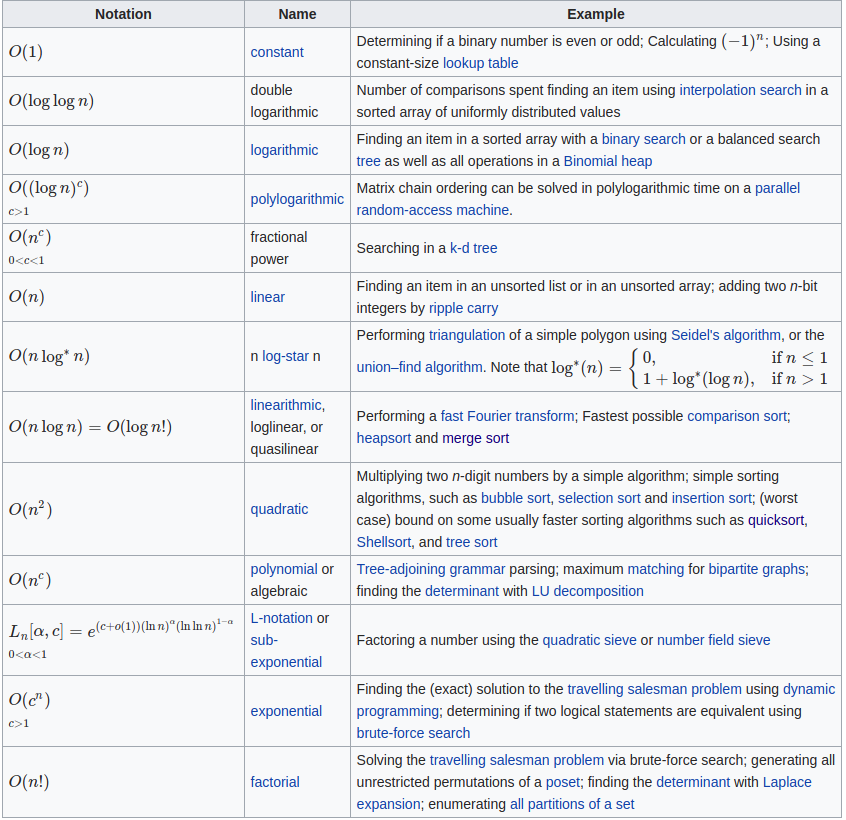
\includegraphics[width= \textwidth]{./Images/classes.png}
\caption{Don't worry about polyarithmitic and L notation. (src. Wikipedia)}
\centering
\end{figure}

\subsection{Fibbonacci Overlapping Subproblems}
\begin{figure}[H]
\caption{Fibbonacci has overlapping subproblems}
\centering
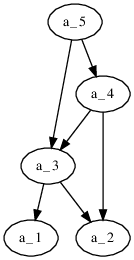
\includegraphics[width=.3\textwidth]{./Images/fibb.png}
\end{figure}



\end{document}
